% =====================================================================
%  Aprendizaje No Supervisado — Sesión 1: Introducción
%  Compilar con: latexmk -pdf Sesion1-Introduccion.tex
%  Figuras: python3 figuras/generar_figuras.py
% =====================================================================
\documentclass[aspectratio=169,11pt]{beamer}

\usepackage[utf8]{inputenc}
\usepackage[T1]{fontenc}
\usepackage[spanish,es-noshorthands,es-nodecimaldot]{babel}
\usepackage{amsmath,amssymb,bm}
\usepackage{booktabs,array}
\usepackage{listings}
\usepackage{tikz}
\usetikzlibrary{positioning,arrows.meta}
\graphicspath{{figuras/}}
\tikzset{b/.style={draw=#1,fill=#1!15,rounded corners,align=center,font=\small,
  minimum width=2.6cm,minimum height=1.6cm}}

% ---------- Tema (común a las presentaciones del curso) ----------
\usetheme{Madrid}
\usefonttheme{professionalfonts}
\definecolor{marino}{HTML}{1F3864}
\definecolor{azul}{HTML}{2E75B6}
\definecolor{naranja}{HTML}{E07B22}
\definecolor{verde}{HTML}{5B9A3C}
\definecolor{fondocod}{HTML}{F4F6F9}
\setbeamercolor{palette primary}{bg=marino,fg=white}
\setbeamercolor{palette secondary}{bg=azul,fg=white}
\setbeamercolor{palette tertiary}{bg=marino,fg=white}
\setbeamercolor{frametitle}{bg=marino,fg=white}
\setbeamercolor{title}{bg=marino,fg=white}
\setbeamercolor{structure}{fg=azul}
\setbeamercolor{block title}{bg=azul,fg=white}
\setbeamercolor{block body}{bg=azul!8}
\setbeamercolor{block title alerted}{bg=naranja,fg=white}
\setbeamercolor{block body alerted}{bg=naranja!10}
\setbeamercolor{block title example}{bg=verde,fg=white}
\setbeamercolor{block body example}{bg=verde!10}
\setbeamercolor{alerted text}{fg=naranja}
\setbeamertemplate{navigation symbols}{}
\setbeamertemplate{itemize items}[circle]
\setbeamertemplate{blocks}[rounded][shadow=false]

\AtBeginSection[]{
  \begin{frame}
    \vfill\centering
    \begin{beamercolorbox}[sep=12pt,center,rounded=true]{title}
      \usebeamerfont{title}\insertsectionhead
    \end{beamercolorbox}
    \vfill
  \end{frame}
}

\lstdefinestyle{py}{
  language=Python, basicstyle=\ttfamily\scriptsize,
  keywordstyle=\color{marino}\bfseries, commentstyle=\color{gray}\itshape,
  stringstyle=\color{naranja}, backgroundcolor=\color{fondocod},
  frame=single, rulecolor=\color{azul!40}, showstringspaces=false,
  columns=fullflexible, breaklines=true, xleftmargin=4pt, xrightmargin=4pt
}
\lstset{style=py}

\newcommand{\R}{\mathbb{R}}
\newcommand{\x}{\bm{x}}
\newcommand{\y}{\bm{y}}

\title[Sesión 1: Introducción]{Sesión 1: Introducción al aprendizaje no supervisado}
\subtitle{Aprendizaje No Supervisado}
\author[A. Espinosa Romero]{Arturo Espinosa Romero}
\institute[FMAT]{Maestría en Inteligencia Artificial \\ Facultad de Matemáticas}
\date{Sesión 1}

% =====================================================================
\begin{document}

\begin{frame}
  \titlepage
\end{frame}

\begin{frame}{Agenda de la sesión}
  \begin{enumerate}
    \item Presentación del curso: competencia, unidades, evaluación y herramientas
    \item Aprendizaje supervisado vs.\ no supervisado
    \item Tipos de problemas no supervisados
    \item Preprocesamiento: valores faltantes, escalamiento y estandarización
    \item Medidas de distancia y similitud
    \item La maldición de la dimensionalidad
    \item Laboratorio: configuración del entorno y exploración de un conjunto de datos sin etiquetas
  \end{enumerate}
\end{frame}

% =====================================================================
\section{Presentación del curso}
% =====================================================================

\begin{frame}{Competencia de la asignatura}
  {\small Introducción práctica al descubrimiento de estructura en datos sin etiquetas:
  dos metodologías básicas ---agrupamiento y reducción de dimensionalidad--- y una
  aplicación práctica: la detección de anomalías.}
  \vspace{2pt}
  \begin{block}{Competencia}
    Implementa modelos de aprendizaje no supervisado mediante técnicas estadísticas y
    algoritmos computacionales para la resolución de problemas de sectores productivos
    y sociales, con evidencia de rigurosidad técnica y sensibilidad respecto a su
    impacto en la toma de decisiones informadas.
  \end{block}
  \vspace{4pt}
  \begin{columns}[T]
    \column{0.48\textwidth}
    \textbf{Datos generales}
    \begin{itemize}
      \item 14 sesiones de 2 horas (28 h presenciales)
      \item 100 h de estudio independiente
      \item 8 créditos, primer semestre
    \end{itemize}
    \column{0.48\textwidth}
    \textbf{Estrategias}
    \begin{itemize}
      \item Aprendizaje basado en problemas
      \item Aprendizaje colaborativo
      \item Aprendizaje basado en retos
    \end{itemize}
  \end{columns}
\end{frame}

\begin{frame}{Requisitos previos y resultados de aprendizaje}
  \begin{columns}[T]
    \column{0.42\textwidth}
    \begin{block}{Requisitos previos (recomendados)}
      \begin{itemize}
        \item Programación introductoria en Python
        \item Estadística y probabilidad básicas
        \item Fundamentos de álgebra lineal
        \item Familiaridad con NumPy / pandas
      \end{itemize}
    \end{block}
    \column{0.54\textwidth}
    \begin{exampleblock}{Al terminar el curso podrás}
      \begin{itemize}
        \item Preparar, escalar y explorar datos reales sin etiquetas
        \item Construir, comparar y validar modelos de agrupamiento
        \item Aplicar e interpretar técnicas de reducción de dimensionalidad
        \item Detectar anomalías con enfoques estadísticos, de densidad y basados en modelos
        \item Entregar un flujo no supervisado completo y comunicar su impacto en la toma de decisiones
      \end{itemize}
    \end{exampleblock}
  \end{columns}
\end{frame}

\begin{frame}{Estructura del curso}
  \centering
  \begin{tikzpicture}[
      >={Stealth}]
    \node[b=gray] (s0) {\textbf{Introducción}\\S1};
    \node[b=azul,right=0.5cm of s0] (u1) {\textbf{Unidad 1}\\Algoritmos de\\agrupamiento\\S2--S6};
    \node[b=naranja,right=0.5cm of u1] (u2) {\textbf{Unidad 2}\\Reducción de\\dimensionalidad\\S7--S10};
    \node[b=red!70!black,right=0.5cm of u2] (u3) {\textbf{Unidad 3}\\Detección de\\anomalías\\S11--S14};
    \foreach \a/\b in {s0/u1,u1/u2,u2/u3} \draw[->,thick,marino] (\a) -- (\b);
  \end{tikzpicture}
  \vspace{10pt}
  \begin{itemize}
    \item Cada sesión: problema detonador, fundamentos, laboratorio guiado, discusión y cierre.
    \item Dos metodologías básicas (agrupar y reducir) y su aplicación: detectar lo atípico.
  \end{itemize}
\end{frame}

\begin{frame}{Evaluación}
  \centering
  \renewcommand{\arraystretch}{1.3}
  \begin{tabular}{@{}lr@{}}
    \toprule
    \textbf{Elemento de evaluación} & \textbf{Peso}\\
    \midrule
    Miniproyecto -- Algoritmos de agrupamiento & 30\,\% \\
    Miniproyecto -- Reducción de dimensionalidad & 35\,\% \\
    Miniproyecto -- Detección de anomalías & 35\,\% \\
    \bottomrule
  \end{tabular}
  \vspace{8pt}
  \begin{block}{Cada miniproyecto}
    Aplica las técnicas de la unidad a un conjunto de datos real de un sector
    productivo o social y discute su impacto en la toma de decisiones.
  \end{block}
\end{frame}

\begin{frame}{Herramientas y bibliografía}
  \begin{columns}[T]
    \column{0.45\textwidth}
    \begin{block}{Software}
      \begin{itemize}
        \item Python 3.10+, JupyterLab o Google Colab
        \item NumPy, SciPy, pandas
        \item scikit-learn, Matplotlib, seaborn
        \item PyOD, PyTorch
        \item Git y GitHub (repositorio de notebooks)
      \end{itemize}
    \end{block}
    \column{0.52\textwidth}
    \begin{block}{Bibliografía básica}
      \small
      \begin{itemize}
        \item James et al.\ (2023). \emph{An Introduction to Statistical Learning with Applications in Python}. Springer.
        \item Bishop (2006). \emph{Pattern Recognition and Machine Learning}. Springer.
        \item Murphy (2022). \emph{Probabilistic Machine Learning: An Introduction}. MIT Press.
      \end{itemize}
    \end{block}
  \end{columns}
\end{frame}

% =====================================================================
\section{Aprendizaje supervisado vs.\ no supervisado}
% =====================================================================

\begin{frame}{Dos formas de aprender de los datos}
  \centering
  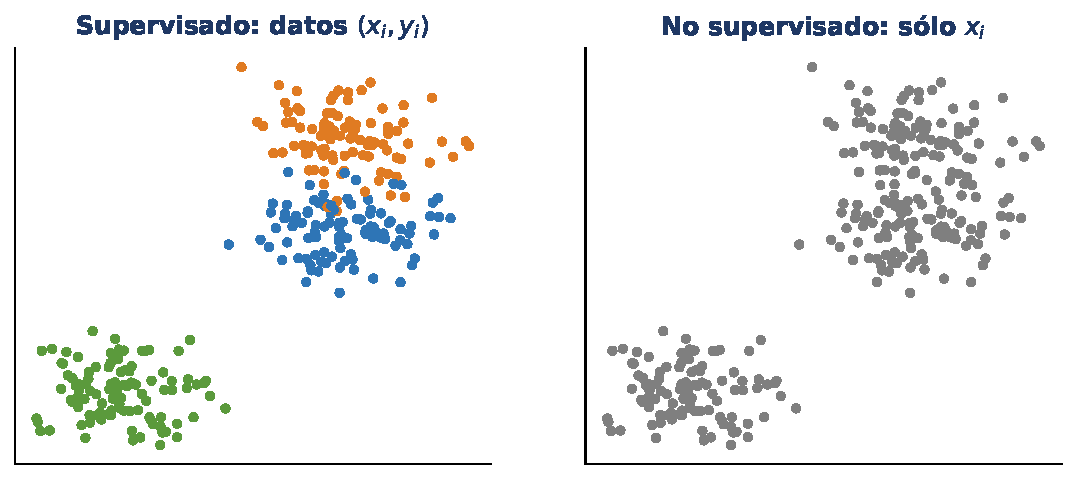
\includegraphics[width=0.8\textwidth]{supervisado_vs_no}
  \begin{columns}[T]
    \column{0.48\textwidth}
    \textbf{Supervisado}: datos $\{(\x_i, y_i)\}_{i=1}^n$.\\
    Aprender $f$ tal que $f(\x)\approx y$.
    \column{0.48\textwidth}
    \textbf{No supervisado}: datos $\{\x_i\}_{i=1}^n$.\\
    Descubrir \alert{estructura} en $p(\x)$.
  \end{columns}
\end{frame}

\begin{frame}{Comparación}
  \renewcommand{\arraystretch}{1.3}
  \begin{tabular}{@{}>{\bfseries}p{0.2\textwidth}>{\raggedright\arraybackslash}p{0.36\textwidth}>{\raggedright\arraybackslash}p{0.36\textwidth}@{}}
    \toprule
    & \textbf{Supervisado} & \textbf{No supervisado}\\
    \midrule
    Datos & Con etiqueta $y$ & Sin etiqueta \\
    Objetivo & Predecir $y$ & Describir la estructura de $\x$ \\
    Evaluación & Error de prueba contra $y$ & Indirecta: índices internos, estabilidad, utilidad, criterio experto \\
    Ejemplos & Regresión, clasificación & Agrupamiento, reducción, anomalías, estimación de densidad \\
    Costo de datos & Etiquetar es caro & Los datos sin etiquetar abundan \\
    \bottomrule
  \end{tabular}
  \vspace{2pt}
  \begin{alertblock}{La dificultad central}
    No hay una ``respuesta correcta'' contra la cual comparar: la validación
    exige rigor técnico y conocimiento del dominio.
  \end{alertblock}
\end{frame}

\begin{frame}{Entre ambos extremos}
  \begin{itemize}
    \item \textbf{Semisupervisado}: pocas etiquetas y muchos datos sin etiquetar.
    \item \textbf{Autosupervisado}: la etiqueta se genera de los propios datos
          (predecir una parte oculta de la entrada); base de los modelos de lenguaje.
    \item \textbf{No supervisado como preprocesamiento}: reducir dimensión o crear rasgos
          (pertenencia a un grupo, puntuación de anomalía) para un modelo supervisado.
  \end{itemize}
 % \vspace{6pt}
 % \begin{exampleblock}{Pregunta para discutir}
 %   Un banco tiene millones de transacciones y sólo unas cientos marcadas como fraude.
 %   ¿Qué enfoque usarías y por qué?
 % \end{exampleblock}
\end{frame}

% =====================================================================
\section{Tipos de problemas no supervisados}
% =====================================================================

\begin{frame}{Tareas principales}
  \renewcommand{\arraystretch}{1.35}
  \begin{tabular}{@{}>{\bfseries}p{0.28\textwidth}>{\raggedright\arraybackslash}p{0.30\textwidth}>{\raggedright\arraybackslash}p{0.34\textwidth}@{}}
    \toprule
    Tarea & Pregunta & Ejemplo \\
    \midrule
    Agrupamiento & ¿Qué grupos naturales existen? & Segmentar clientes \\
    Reducción de dimensionalidad & ¿Cómo describo los datos con menos variables? & Visualizar perfiles de expresión génica \\
    Detección de anomalías & ¿Qué observaciones son raras? & Fraude, fallas en sensores \\
    Estimación de densidad & ¿Cuál es la distribución $p(\x)$? & Modelar el consumo eléctrico \\
    Reglas de asociación & ¿Qué variables ocurren juntas? & Análisis de canasta de compra \\
    \bottomrule
  \end{tabular}
  \vspace{4pt}
  {\small Las tres primeras son las unidades del curso, en ese orden.}
\end{frame}

\begin{frame}{Aplicaciones en sectores productivos y sociales}
  \begin{columns}[T]
    \column{0.48\textwidth}
    \begin{block}{Productivos}
      \begin{itemize}
        \item Segmentación de clientes y mercados
        \item Mantenimiento predictivo en la industria
        \item Detección de fraude financiero
        \item Control de calidad con imágenes
      \end{itemize}
    \end{block}
    \column{0.48\textwidth}
    \begin{block}{Sociales}
      \begin{itemize}
        \item Tipologías de hogares con datos censales
        \item Detección de brotes epidemiológicos
        \item Análisis temático de textos y redes sociales
        \item Zonificación urbana y de marginación
      \end{itemize}
    \end{block}
  \end{columns}
  \vspace{6pt}
  \begin{alertblock}{Impacto en decisiones}
    Un grupo o una anomalía se convierte en una acción (una campaña, una auditoría, una
    política pública). Errores y sesgos tienen consecuencias reales.
  \end{alertblock}
\end{frame}

\begin{frame}{Flujo de trabajo típico}
  \centering
  \begin{tikzpicture}[
      p/.style={draw=azul,fill=azul!10,rounded corners,align=center,font=\small,
                minimum width=2.3cm,minimum height=1.1cm},
      >={Stealth}]
    \node[p] (a) {Entender el\\problema};
    \node[p,right=0.4cm of a] (b) {Explorar\\los datos};
    \node[p,right=0.4cm of b] (c) {Preprocesar};
    \node[p,right=0.4cm of c] (d) {Modelar};
    \node[p,right=0.4cm of d] (e) {Validar e\\interpretar};
    \node[p,fill=naranja!15,draw=naranja,right=0.4cm of e] (f) {Decidir y\\comunicar};
    \foreach \u/\v in {a/b,b/c,c/d,d/e,e/f} \draw[->,thick,marino] (\u) -- (\v);
    \draw[->,thick,marino,dashed] (e.south) to[bend left=25] node[below,font=\scriptsize]{iterar} (c.south);
  \end{tikzpicture}
  \vspace{8pt}
  \begin{itemize}
    \item Sin etiquetas, el preprocesamiento y la elección de la distancia \alert{determinan} el resultado.
    \item La validación combina métricas, estabilidad y criterio experto.
  \end{itemize}
\end{frame}

% =====================================================================
\section{Preprocesamiento}
% =====================================================================

%\begin{frame}{Valores faltantes}
%  \textbf{Mecanismos} (Rubin):
%  \begin{itemize}
%    \item \textbf{MCAR}: falta completamente al azar.
%    \item \textbf{MAR}: depende de otras variables observadas.
%    \item \textbf{MNAR}: depende del propio valor faltante (p.\ ej., ingresos %altos no reportados).
%  \end{itemize}
%  \vspace{4pt}
%  \renewcommand{\arraystretch}{1.25}
%  %\begin{tabular}{@{}>{\raggedright\arraybackslash}p{0.3\textwidth}>{\raggedright\arraybackslash}p{0.62\textwidth}@{}}
%    \toprule
%    \textbf{Estrategia} & \textbf{Comentario}\\
%    \midrule
%    Eliminar filas o columnas & Simple; pierde información y puede sesgar si  no es MCAR \\
%    Media / mediana / moda & Rápida; reduce la varianza y distorsiona correlaciones \\
%    kNN (\texttt{KNNImputer}) & Usa observaciones similares; depende de la distancia \\ 
%    Iterativa (\texttt{IterativeImputer}) & Modela cada variable a partir de las demás \\
%     Indicador de faltante & Conserva la información de que el dato faltaba \\
%     \bottomrule
%   \end{tabular}
% \end{frame}

\begin{frame}{¿Por qué escalar? Un ejemplo con k-medias}
  \centering
  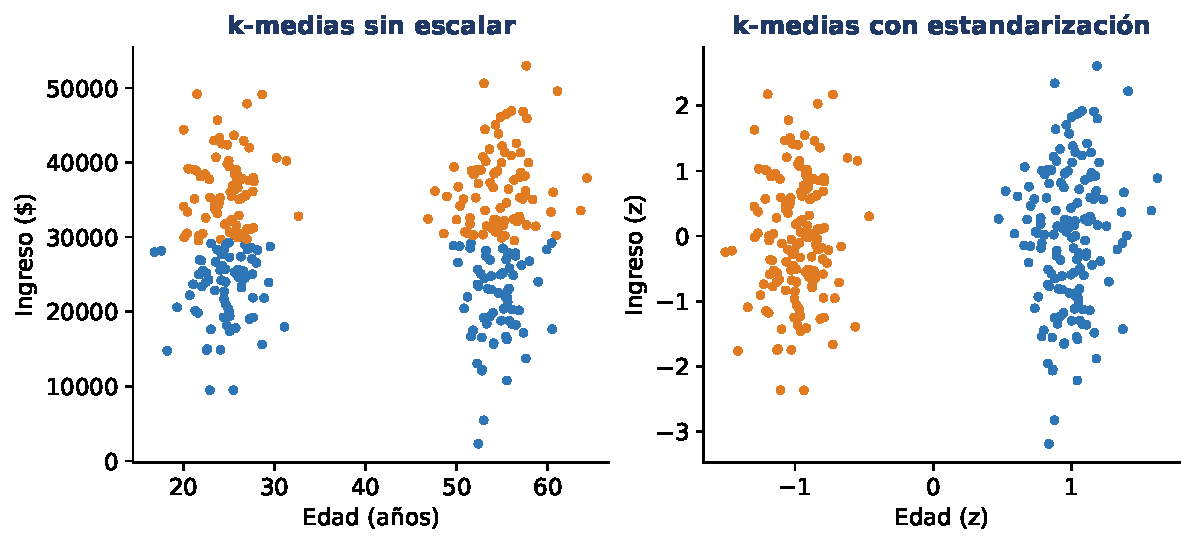
\includegraphics[width=0.85\textwidth]{efecto_escala}
  \begin{itemize}
    \item Los grupos reales difieren en \textbf{edad}, pero el \textbf{ingreso} se mide en miles.
    \item Sin escalar, la distancia la domina el ingreso y k-medias corta en la dirección equivocada.
  \end{itemize}
\end{frame}



\begin{frame}{Transformaciones de escala}
  \renewcommand{\arraystretch}{1.5}
  \footnotesize
  \begin{tabular}{@{}lll@{}}
    \toprule
    \textbf{Método} & \textbf{Fórmula} & \textbf{Propiedad}\\
    \midrule
    Estandarización (\texttt{StandardScaler}) & $z = \dfrac{x - \bar{x}}{s}$ & Media 0, varianza 1 \\
    Mín--máx (\texttt{MinMaxScaler}) & $z = \dfrac{x - x_{\min}}{x_{\max} - x_{\min}}$ & Rango $[0,1]$ \\
    Robusta (\texttt{RobustScaler}) & $z = \dfrac{x - \operatorname{mediana}}{\operatorname{IQR}}$ & Resistente a atípicos \\
    Norma unitaria (\texttt{Normalizer}) & $\x \leftarrow \x / \lVert\x\rVert$ & Por fila; útil con coseno \\
    \bottomrule
  \end{tabular}
  \vspace{2pt}
  \centering
  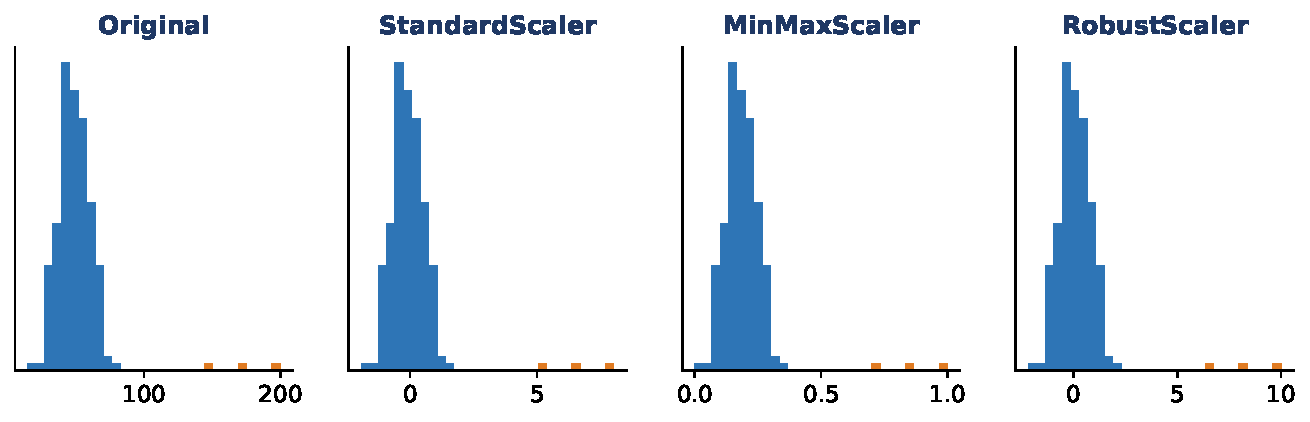
\includegraphics[height=0.4\textheight]{escaladores}
\end{frame}

\begin{frame}{Otras transformaciones}
  \begin{itemize}
    \item \textbf{Variables sesgadas}: logaritmo, Box-Cox, Yeo-Johnson (\texttt{PowerTransformer}).
    \item \textbf{Categóricas}: codificación one-hot; cuidado con su peso en la distancia.
    \item \textbf{Mixtas}: distancia de Gower o separar el análisis.
    \item \textbf{Atípicos}: decidir si son ruido o el fenómeno de interés (Unidad 3).
  \end{itemize}
  \vspace{6pt}
  \begin{alertblock}{Regla práctica}
    Ajustar las transformaciones dentro de un \texttt{Pipeline} y documentar cada decisión:
    en no supervisado cambian el resultado tanto como el algoritmo.
  \end{alertblock}
\end{frame}

% =====================================================================
\section{Medidas de distancia y similitud}
% =====================================================================

\begin{frame}{Propiedades de una métrica}
  Una función $d(\x,\y)$ es una \textbf{métrica} si para todo $\x,\y,\bm{z}$:
  \begin{enumerate}
    \item $d(\x,\y) \ge 0$ \hfill (no negatividad)
    \item $d(\x,\y) = 0 \iff \x = \y$ \hfill (identidad)
    \item $d(\x,\y) = d(\y,\x)$ \hfill (simetría)
    \item $d(\x,\bm{z}) \le d(\x,\y) + d(\y,\bm{z})$ \hfill (desigualdad del triángulo)
  \end{enumerate}
  \vspace{6pt}
  \begin{block}{Distancia vs.\ similitud}
    Una \textbf{similitud} $s(\x,\y)$ es grande cuando los objetos se parecen.
    Se convierten, por ejemplo, con $d = 1 - s$ o $s = \exp(-\gamma d^2)$.
  \end{block}
\end{frame}

\begin{frame}{Distancias de Minkowski}
  \begin{columns}[c]
    \column{0.55\textwidth}
    \[
      d_p(\x,\y) = \Bigl(\sum_{j=1}^{d}\lvert x_j - y_j\rvert^p\Bigr)^{1/p}
    \]
    \begin{itemize}
      \item $p = 1$: \textbf{Manhattan}, $\sum_j |x_j - y_j|$; menos sensible a diferencias grandes en una variable.
      \item $p = 2$: \textbf{Euclidiana}; la más usada (k-medias, PCA).
      \item $p\to\infty$: \textbf{Chebyshev}, $\max_j |x_j - y_j|$.
    \end{itemize}
    \column{0.4\textwidth}
    \centering
    \begin{tikzpicture}[scale=1.5]
      \draw[->,gray] (-1.3,0) -- (1.3,0);
      \draw[->,gray] (0,-1.3) -- (0,1.3);
      \draw[thick,naranja] (1,0) -- (0,1) -- (-1,0) -- (0,-1) -- cycle;
      \draw[thick,azul] (0,0) circle (1);
      \draw[thick,verde] (-1,-1) rectangle (1,1);
      \node[naranja,font=\scriptsize] at (0.25,0.35) {$p=1$};
      \node[azul,font=\scriptsize] at (0.95,0.65) {$p=2$};
      \node[verde,font=\scriptsize] at (1.0,1.15) {$p=\infty$};
    \end{tikzpicture}\\
    {\small Puntos a distancia 1 del origen}
  \end{columns}
\end{frame}

\begin{frame}{Distancia de Mahalanobis}
  \begin{columns}[c]
    \column{0.52\textwidth}
    \[
      d_M(\x,\y) = \sqrt{(\x-\y)^\top \bm{\Sigma}^{-1}(\x-\y)}
    \]
    \begin{itemize}
      \item Toma en cuenta la \alert{escala y la correlación} de las variables.
      \item Con $\bm{\Sigma} = \mathbf{I}$ es la euclidiana; con $\bm{\Sigma}$ diagonal equivale a estandarizar.
      \item A y B están a la misma distancia euclidiana del centro, pero B es mucho más atípico.
      \item Se usará en detección de anomalías (Unidad 3).
    \end{itemize}
    \column{0.45\textwidth}
    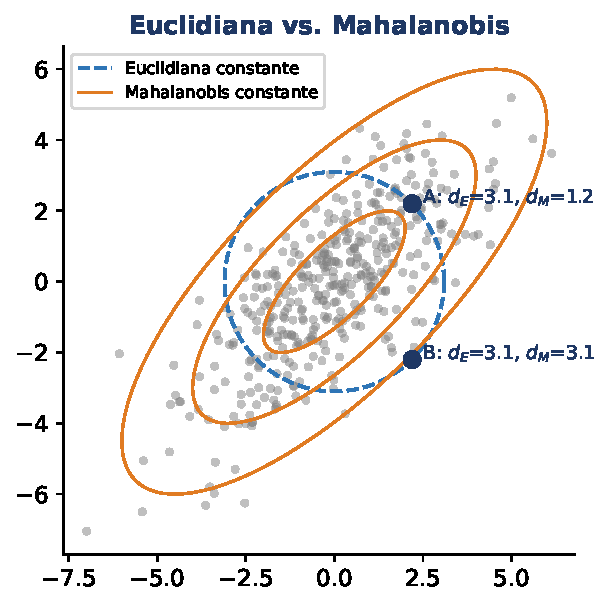
\includegraphics[width=\textwidth]{mahalanobis}
  \end{columns}
\end{frame}

\begin{frame}{Similitud coseno y otras medidas}
  \[
    s_{\cos}(\x,\y) = \frac{\x^\top\y}{\lVert\x\rVert\,\lVert\y\rVert} \in [-1,1],
    \qquad d_{\cos} = 1 - s_{\cos}
  \]
  \begin{itemize}
    \item Mide el \textbf{ángulo}, no la magnitud: dos documentos con el mismo tema pero distinta longitud son similares.
    \item Estándar en texto (TF-IDF) y en \emph{embeddings}.
  \end{itemize}
  \vspace{4pt}
  \renewcommand{\arraystretch}{1.25}
  \begin{tabular}{@{}lll@{}}
    \toprule
    \textbf{Medida} & \textbf{Fórmula} & \textbf{Datos}\\
    \midrule
    Jaccard & $|A\cap B| / |A\cup B|$ & Conjuntos, binarios \\
    Hamming & número de posiciones distintas & Categóricos, cadenas \\
    Correlación & $1 - r(\x,\y)$ & Perfiles, series de tiempo \\
    Gower & promedio de distancias por tipo de variable & Datos mixtos \\
    \bottomrule
  \end{tabular}
\end{frame}

\begin{frame}{Ejercicio: elegir la distancia}
  \begin{exampleblock}{Calcula}
    Sea $\x = (1, 2, 3)$ y $\y = (2, 4, 6)$.
    \begin{enumerate}
      \item Distancias euclidiana, Manhattan y Chebyshev.
      \item Similitud coseno. ¿Qué observas?
    \end{enumerate}
  \end{exampleblock}
  \pause
  \begin{block}{Solución}
    $d_2 = \sqrt{1+4+9} = \sqrt{14}\approx 3.74$; \quad $d_1 = 6$; \quad $d_\infty = 3$.\\
    $s_{\cos} = 28 / (\sqrt{14}\cdot\sqrt{56}) = 1$: misma dirección; $\y = 2\x$.
  \end{block}
  \begin{alertblock}{Para discutir}
    ¿Qué distancia usarías para comparar canastas de compra? ¿Y perfiles de clientes con edad e ingreso?
  \end{alertblock}
\end{frame}

% =====================================================================
\section{La maldición de la dimensionalidad}
% =====================================================================

\begin{frame}{Qué ocurre en alta dimensión}
  \centering
  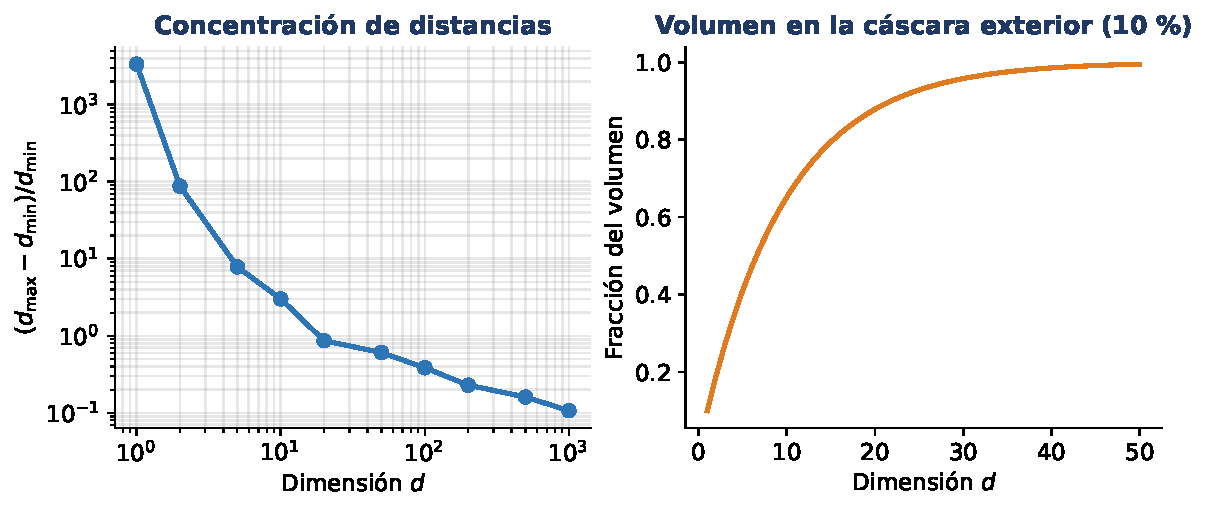
\includegraphics[width=0.85\textwidth]{maldicion}
  \begin{itemize}
    \item \textbf{Concentración de distancias}: el vecino más cercano y el más lejano casi equidistan.
    \item \textbf{Volumen en la frontera}: en el hipercubo, la fracción en la cáscara exterior es $1-0.9^d$; con $d=50$ es 99\,\%.
  \end{itemize}
\end{frame}

\begin{frame}{Consecuencias y remedios}
  \begin{columns}[T]
    \column{0.48\textwidth}
    \begin{alertblock}{Consecuencias}
      \begin{itemize}
        \item Los datos se vuelven dispersos.
        \item Agrupamiento (Unidad 1) y kNN pierden poder discriminante.
        \item Densidades difíciles de estimar.
        \item Se requieren muchos más datos.
      \end{itemize}
    \end{alertblock}
    \column{0.48\textwidth}
    \begin{exampleblock}{Remedios}
      \begin{itemize}
        \item Reducción de dimensionalidad (Unidad 2).
        \item Selección de variables relevantes.
        \item Distancias adecuadas (coseno en texto).
        \item Aprovechar la baja dimensión intrínseca de los datos reales.
      \end{itemize}
    \end{exampleblock}
  \end{columns}
  \vspace{6pt}
  {\small Ejemplo: para tener 10 puntos por eje en $[0,1]^d$ se necesitan $10^d$ observaciones.}
\end{frame}

% 
% =====================================================================
\section{Laboratorio}
% =====================================================================

\begin{frame}[fragile]{Configuración del entorno}
\begin{lstlisting}[language=bash]
# Opcion A: conda
conda create -n ans python=3.12
conda activate ans
pip install numpy scipy pandas scikit-learn matplotlib seaborn jupyterlab umap-learn pyod

# Opcion B: uv
uv venv && source .venv/bin/activate
uv pip install numpy scipy pandas scikit-learn matplotlib seaborn jupyterlab umap-learn pyod

# Verificar
python -c "import sklearn; print(sklearn.__version__)"
jupyter lab
\end{lstlisting}
  \small Alternativa sin instalación: Google Colab. Crear un repositorio en GitHub para los notebooks del curso.
\end{frame}

\begin{frame}[fragile]{Exploración de un conjunto de datos sin etiquetas}
\begin{lstlisting}
import pandas as pd
from sklearn.datasets import load_wine
from sklearn.pipeline import make_pipeline
from sklearn.impute import SimpleImputer
from sklearn.preprocessing import StandardScaler
from sklearn.metrics import pairwise_distances

df = load_wine(as_frame=True).data           # ignoramos la etiqueta a proposito
print(df.shape); print(df.describe().T)      # escalas muy distintas
print(df.isna().mean())                      # proporcion de faltantes

prep = make_pipeline(SimpleImputer(strategy="median"), StandardScaler())
X = prep.fit_transform(df)

for metrica in ["euclidean", "manhattan", "cosine"]:
    D = pairwise_distances(X, metric=metrica)
    print(metrica, D.mean().round(2))

df.corr().style.background_gradient(cmap="coolwarm")  # correlaciones
\end{lstlisting}
\end{frame}

\begin{frame}{Actividad y tarea}
  \begin{block}{En clase}
    \begin{enumerate}
      \item Instalar el entorno y crear el repositorio de notebooks.
      \item Explorar el conjunto de vinos: escalas, faltantes, correlaciones, histogramas.
      \item Comparar los 5 vecinos más cercanos de una observación con y sin estandarizar, usando distancia euclidiana y coseno.
    \end{enumerate}
  \end{block}
  \begin{exampleblock}{Para la sesión 2}
    \begin{itemize}
      \item Subir el notebook de la sesión al repositorio.
      \item Leer: James et al.\ (2023), cap.~12.1 y 12.4.1 (k-medias); Bishop (2006), cap.~9.1.
      \item Repasar distancia euclidiana y estandarización: k-medias depende de ambas.
    \end{itemize}
  \end{exampleblock}
\end{frame}


\begin{frame}{Resumen}
  \begin{itemize}
    \item El aprendizaje no supervisado busca estructura en datos sin etiquetas.
    \item Tareas del curso: agrupamiento, reducción de dimensionalidad y detección de anomalías.
    \item Sin etiquetas, \alert{el preprocesamiento y la distancia definen el resultado}.
    \item Estandarizar cuando las unidades difieren; elegir la distancia según el tipo de datos.
    \item En alta dimensión las distancias pierden contraste: motivo de la Unidad 2.
  \end{itemize}
\end{frame}

\end{document}
